\section{Моделирование движения двух космических аппаратов как двух материальных точек при действии тяги на одном из них}
\label{SEC:2SPH}

В этом разделе рассмотрим случай, в котором расстояние между пассивным и активным аппаратами изменяется за счет тяги на активном аппарате.
Аппараты представлены как материальные точки, между которыми происходит электростатическое взаимодействие (рис. \ref{ris:2sph}).

\begin{figure}[H]
	\center{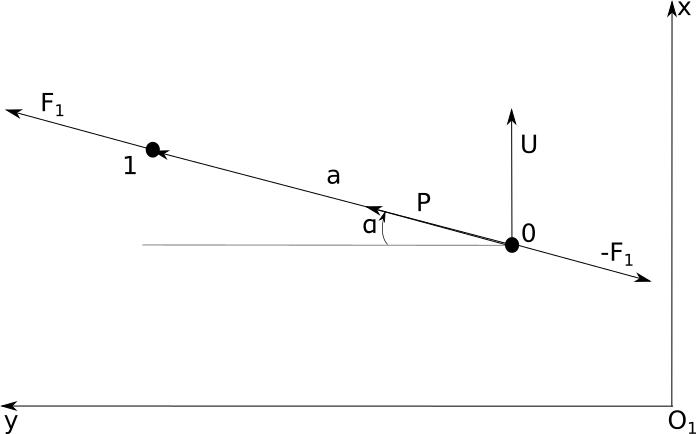
\includegraphics[scale=0.75]{2sph.png}}
	\caption{Замена космических аппаратов двумя материальными точками}
	\label{ris:2sph}
\end{figure}

Определим положения тел векторами $\vec{r}_0$ и $\vec{r}_1$:
\begin{equation}
\label{eq:2sph_r0}
	\vec{r}_0 = 
	\begin{pmatrix}
		x\\
		y
	\end{pmatrix},
\end{equation}
\begin{equation}
\label{eq:2sph_r1}
	\vec{r}_1 = \vec{r}_0 + \vec{A},
\end{equation}
где $A$ – вектор между материальными точками:
\begin{equation}
\label{eq:2sph_A}
	\vec{A} = 
	\begin{pmatrix}
		- a \sin \alpha \\
		a \cos \alpha
	\end{pmatrix},
\end{equation}
где $a$ – расстояние между аппаратами, $\alpha$ – угол между вектором $A$ и осью $OY$.

Скорости тел:
\begin{equation}
\label{eq:2sph_v0}
	\vec{v}_0 = \frac{d \vec{r}_0}{dt},
\end{equation}
\begin{equation}
\label{eq:2sph_v1}
	\vec{v}_1 = \frac{d \vec{r}_1}{dt}.
\end{equation}

Запишем кинетическую энергию системы:
\begin{equation}
\label{eq:2sph_T}
	T = m_0 \frac{\norm{\vec{v}_0}^2}{2} + m_1 \frac{\norm{\vec{v}_1}^2}{2},
\end{equation}
где $m_0$ – масса активного аппарата, $m_1$ – масса пассивного аппарата.

Сила кулоновского взаимодействия:
\begin{equation}
\label{eq:2sph_f1}
	\vec{F}_1 = \frac{n}{a^3}\vec{A},
\end{equation}
где $n = k_c q_0 q_1$.

Сила, действующая на активный аппарат:
\begin{equation}
\label{eq:2sph_f0}
	\vec{F}_0 = \vec{P} - \vec{F}_1,
\end{equation}
где $\vec{F}_1$ – сила кулоновского взаимодействия (\ref{eq:2sph_f1}), $\vec{P}$ – вектор тяги:
\begin{equation}
\label{eq:2sph_P}
	\vec{P} = \frac{p}{a} \vec{A},
\end{equation}
где $p$ – тяга.

Обобщенными координаты:
\begin{equation}
\label{eq:2sph_qj}
	\begin{pmatrix}
		q_x \\
		q_y \\
		q_a \\
		q_\alpha \\
	\end{pmatrix} 
	=
	\begin{pmatrix}
		x \\
		y \\
		a \\
		\alpha \\
	\end{pmatrix}.
\end{equation}

Обобщенные силы будут иметь вид:
\begin{equation}
\label{eq:2sph_Q}
	Q_j = \frac{\partial r_0}{\partial q_j} \cdot F_0 + \frac{\partial r_1}{\partial q_j} \cdot F_1,
\end{equation}
где $q_j$ – обобщенные координаты.

Подставив (\ref{eq:2sph_r0}) - (\ref{eq:2sph_Q}) в уравнение Лагранжа второго рода (\ref{eq:3sph_lag}) и численно решив получившуюся систему найдем зависимости $x$, $y$, $a$, $\alpha$ от времени.
Зададим параметры системы $m_0 = 200$кг, $m_1=1000$кг, $p=0.2$H, $n=8.3 * 10^{-3}$.
Начальные условия:
\begin{equation}
	\begin{cases}
		x(0) = 0, \\
		y(0) = 0, \\
		a(0) = 5.4, \\
		\alpha(0) = 0,\\
		x'(0) = 0, \\
		y'(0) = 0, \\
		a'(0) = 0, \\
		\alpha'(0) = 0.01.
	\end{cases}
\end{equation}

Решение изображено на рисунках \ref{ris:2sph_a_no_u} - \ref{ris:2sph_y_no_u}.

\begin{figure}[H]
	\center{\includegraphics[scale=0.7]{2sph_no_u_a.png}}
	\caption{Зависимость координаты $a$ от времени $t$}
	\label{ris:2sph_a_no_u}
\end{figure}
\begin{figure}[H]
	\center{\includegraphics[scale=0.7]{2sph_no_u_alpha.png}}
	\caption{Зависимость координаты $\alpha$ от времени $t$}
	\label{ris:2sph_alpha_no_u}
\end{figure} 
\begin{figure}[H]
	\center{\includegraphics[scale=0.7]{2sph_no_u_x.png}}
	\caption{Зависимость координаты $x$ от времени $t$}
	\label{ris:2sph_x_no_u}
\end{figure} 
\begin{figure}[H]
	\center{\includegraphics[scale=0.7]{2sph_no_u_y.png}}
	\caption{Зависимость координаты $y$ от времени $t$}
	\label{ris:2sph_y_no_u}
\end{figure} 

Как видно из рисунка \ref{ris:2sph_alpha_no_u} активный аппарат начинает вращаться вокруг пассивного.
Для предотвращения этого нам нужно с помощью введения управления получить для $\alpha$ уравнение периодического вида (уравнение маятника с демпфированием).

Введем управляющую тягу $U$, направленную перпендикулярно к тяге $P$:
\begin{equation}
\label{ris:2sph_U_alpha}
	\vec{U} = 
	\begin{pmatrix}
		\cos \alpha \left(k_\alpha \sin \alpha + k_{\alpha t}\alpha'\right)\\
		\sin \alpha \left(k_\alpha \sin \alpha + k_{\alpha t}\alpha'\right)
	\end{pmatrix}.
\end{equation}

$\vec{F}_0$ (\ref{eq:2sph_f0}) примет вид:
\begin{equation}
\label{eq:2sph_f0_u}
	\vec{F}_0 = \vec{P} - \vec{F}_1 + \vec{U}.
\end{equation}

Результаты численного моделирования для управляемого движения при $k_\alpha = -5$ и $k_{\alpha t} = -2$ изображены на рисунках \ref{ris:2sph_a_alpha_u} - \ref{ris:2sph_y_alpha_u}.

\begin{figure}[H]
	\center{\includegraphics[scale=0.7]{2sph_alpha_u_a.png}}
	\caption{Зависимость координаты $a$ от времени $t$ с управлением по $\alpha$}
	\label{ris:2sph_a_alpha_u}
\end{figure}
\begin{figure}[H]
	\center{\includegraphics[scale=0.7]{2sph_alpha_u_alpha.png}}
	\caption{Зависимость координаты $\alpha$ от времени $t$ с управлением по $\alpha$}
	\label{ris:2sph_alpha_alpha_u}
\end{figure} 
\begin{figure}[H]
	\center{\includegraphics[scale=0.7]{2sph_alpha_u_x.png}}
	\caption{Зависимость координаты $x$ от времени $t$ с управлением по $\alpha$}
	\label{ris:2sph_x_alpha_u}
\end{figure} 
\begin{figure}[H]
	\center{\includegraphics[scale=0.7]{2sph_alpha_u_y.png}}
	\caption{Зависимость координаты $y$ от времени $t$ с управлением по $\alpha$}
	\label{ris:2sph_y_alpha_u}
\end{figure} 

Как видно из рисунков \ref{ris:2sph_a_alpha_u} и \ref{ris:2sph_alpha_alpha_u} с управлением по $\alpha$ со временем координаты $a$ и $\alpha$ стабилизируются.
Но аппараты продолжают расходиться по координате $x$.
Для решения этой проблемы поступим аналогичным образом с $x$.

Введем новую управляющую тягу $U$:
\begin{equation}
\label{eq:2sph_u_full}
	\vec{U} = 
	\begin{pmatrix}
		\cos \alpha \left(k_\alpha \sin \alpha + k_{\alpha t}\alpha' + k_x x + x_{xt} x'\right)\\
		\sin \alpha \left(k_\alpha \sin \alpha + k_{\alpha t}\alpha' + k_x x + x_{xt} x'\right)
	\end{pmatrix}.
\end{equation}

Результаты численного моделирования для управляемого движения с $U$ (\ref{eq:2sph_u_full}) при $k_\alpha = -5$,$k_{\alpha t} = -2$,$k_x = 0.1$,$k_{x t} = 0.1$ изображены на рисунках \ref{ris:2sph_a_full_u} - \ref{ris:2sph_y_full_u}.

\begin{figure}[H]
	\center{\includegraphics[scale=0.7]{2sph_full_u_a.png}}
	\caption{Зависимость координаты $a$ от времени $t$ с управлением по $\alpha$ и $x$}
	\label{ris:2sph_a_full_u}
\end{figure}
\begin{figure}[H]
	\center{\includegraphics[scale=0.7]{2sph_full_u_alpha.png}}
	\caption{Зависимость координаты $\alpha$ от времени $t$ с управлением по $\alpha$ и $x$}
	\label{ris:2sph_alpha_full_u}
\end{figure} 
\begin{figure}[H]
	\center{\includegraphics[scale=0.7]{2sph_full_u_x.png}}
	\caption{Зависимость координаты $x$ от времени $t$ с управлением по $\alpha$ и $x$}
	\label{ris:2sph_x_full_u}
\end{figure} 
\begin{figure}[H]
	\center{\includegraphics[scale=0.7]{2sph_full_u_y.png}}
	\caption{Зависимость координаты $y$ от времени $t$ с управлением по $\alpha$ и $x$}
	\label{ris:2sph_y_full_u}
\end{figure} 

С введением такого управления (\ref{eq:2sph_u_full}) координаты $x$, $y$, $a$ и $\alpha$ стремятся к своим устойчивым положениям: $x$ колеблется около 0, $y$ растет,  $a$ колеблется около $0.5$, $\alpha$ колеблется около 0.
